\documentclass[11pt,a4paper]{article}
\usepackage[margin=2.6cm]{geometry}
\usepackage[T1]{fontenc}
\usepackage{lmodern}
\usepackage[letterspace=180]{microtype}
\usepackage{booktabs}
\usepackage{amsmath}
\usepackage{parskip}
\usepackage{xcolor}
\usepackage[most]{tcolorbox}
\usepackage{titlesec}
\usepackage{caption}
\usepackage{graphicx}

\definecolor{bcnavy}{RGB}{24,38,68}
\definecolor{bcgold}{RGB}{198,160,74}
\definecolor{bcteal}{RGB}{23,110,120}
\definecolor{bcgrey}{RGB}{95,95,95}
\definecolor{bcred}{RGB}{160,60,50}

\titleformat{\section}{\bfseries\large\color{bcnavy}}{\thesection.}{0.6em}{}
\titleformat{\subsection}{\bfseries\color{bcteal}}{}{0em}{}
\captionsetup{font={footnotesize},labelformat=empty,textfont={color=bcgrey}}
\newcommand{\tabnote}[1]{\begin{center}\begin{minipage}{0.92\textwidth}
  \footnotesize\color{bcgrey}#1\end{minipage}\end{center}}
\newcommand{\good}[1]{{\color{bcteal}\textbf{#1}}}
\newcommand{\bad}[1]{{\color{bcred}\textbf{#1}}}

\begin{document}

% ---------------------------------------------------------------- cover
\begin{titlepage}
\centering
\vspace*{3.2cm}

\includegraphics[width=5cm]{bc_logo.pdf}

\vspace{1.6cm}
{\color{bcnavy}\rule{7cm}{0.6pt}}

\vspace{0.9cm}
{\LARGE\bfseries\color{bcnavy} Bear-Market Protection\\[0.15cm] for the Nine-Name Book\par}
\vspace{0.35cm}
{\large\color{bcnavy} Three defensive mechanisms priced on real bear data:\\
the per-stock stop, the book-wide circuit breaker,\\
and the 200-day moving-average gate\par}

\vspace{0.9cm}
{\color{bcgold}\rule{7cm}{1.0pt}}

\vspace{1.5cm}
{\bfseries Bayesian Capital}\\[0.2cm]
{\color{bcgrey} Systematic Trading Research}\\[0.9cm]
{\itshape\color{bcgrey} Internal document --- strictly confidential}\\[0.3cm]
{\color{bcgrey} 15 August 2026 --- gate adopted and wired the same day (\S7);\\execution-accurate restatement added 19 August (\S8);\\breadth upgrade adopted and wired 26 August (\S9)}
\vfill
\end{titlepage}

% ---------------------------------------------------------------- header
\begin{center}
{\Large\bfseries\color{bcnavy} Bear-Market Protection for the Nine-Name Book}\\[0.15cm]
{\color{bcnavy} per-stock stop $\cdot$ book-wide circuit breaker $\cdot$ 200-day
moving-average gate}\\[0.25cm]
{\small\color{bcgrey} Bayesian Capital --- Systematic Trading Research
\;$\bullet$\; book: TSM $\cdot$ VRT $\cdot$ VST $\cdot$ AVGO $\cdot$ MU
$\cdot$ GM $\cdot$ VLO $\cdot$ CF $\cdot$ MRVL \;$\bullet$\; all figures on verified fills}
\end{center}
\vspace{0.1cm}
{\color{bcnavy}\hrule height 0.8pt}
\vspace{0.5cm}

\section{The question, and the data that finally answers it}

Every result the book stands on was measured between April 2024 and August 2026
--- a bull market. The strategy buys volatility dips below a trend-following (Bayes)
or mean-reverting (OU) fair value and sells a quick fixed premium; every panic in
that sample mean-reverted, so every study rewarded staying fully engaged and
punished every protective overlay. The one question that sample cannot answer is
the one that matters most: \textbf{what happens when the trend flattens and
reverses --- and what should the book do about it?}

This paper answers it with real bear data. Five-minute bars were obtained for all
nine names covering August 2021 -- June 2023, so the deployed configuration ---
every parameter exactly as it trades today, fitted only on 2024--26 data --- was
replayed through calendar 2022, a year in which the book's AI names fell 40--80\%.
The replay runs on the same verified-fill standard as every other result (a
same-day round trip is booked only where the 5-minute bars prove the low reached
the bid before the high reached the target). Three protective mechanisms are then
priced on both sides: what each \emph{costs} in the 2024--26 bull sample, and what
each \emph{saves} in the 2022 bear.

\subsection{The unprotected baseline: how the book actually loses}

Nothing in the deployed design resists a sustained downtrend. Both fair-value
anchors follow the price down with a lag, so the bids keep filling all the way
down; the ATH cap goes slack immediately (price is far below any peak); the
50-calendar-day time stop is the only loss-taking exit, so damage arrives in
50-day quanta at full sleeve size; and the free-sleeve pooling --- worth
$+2.7$pp in a bull market --- recycles every stop's proceeds into another falling
name's bid the next morning. Calendar 2022, per name:

\begin{center}
\begin{tabular}{lrrrr}
\toprule
name & buy \& hold 2022 & model 2022 & model max DD & time stops \\
\midrule
TSM  & $-42.2\%$ & $-36.2\%$ & 48\% & 8 \\
VRT  & $-44.0\%$ & $-36.4\%$ & 58\% & 7 \\
VST  & $+2.0\%$  & \good{$+29.4\%$} & 17\% & 4 \\
RKLB & $-69.1\%$ & $-69.4\%$ & 71\% & 8 \\
MU   & $-47.8\%$ & $-38.3\%$ & 42\% & 8 \\
GM   & $-45.0\%$ & $-31.6\%$ & 43\% & 7 \\
VLO  & $+64.4\%$ & $+29.1\%$ & 30\% & 3 \\
CF   & $+20.6\%$ & \good{$+49.0\%$} & 19\% & 3 \\
MRVL & $-58.6\%$ & $-58.0\%$ & 61\% & 10 \\
\bottomrule
\end{tabular}
\end{center}

\tabnote{Deployed 2024--26 parameters driven backwards through Aug 2021 -- Jun 2023;
verified fills from the 5-minute bars; calendar-2022 window. Note the stop counts:
3--10 per name in one year, against 1--3 per name across the entire 2.35-year bull
sample.}

Two structural facts stand out. On falling names the model tracks the decline
almost one-for-one (RKLB $-69\%$ vs $-69\%$): it stops out, re-enters the next
dip, and rides the next leg down --- the \emph{re-entry treadmill}. But on the
names that went sideways-to-up, dip-buying had an excellent year: the model beat
buy-and-hold by 27pp on VST and 28pp on CF. The diversifiers earned their seats
in precisely the scenario they were admitted for. At book level (pooled, equal
weights) the unprotected 2022 outcome is \textbf{$-21.9\%$ with a 28.1\% maximum
drawdown} --- painful, but survivable, and no deeper than the April 2025 tariff
episode the live book has already been through.

\section{Mechanism 1: the per-stock stop}

\subsection{What it is}

A stop-loss on each position: exit at $\text{entry} \times (1-f)$ whenever the
price gets there before the 50-day time stop. Modelled with honest execution:
filled at the stop level, at the open if the session gaps below it, and if the
take-profit target and the stop level are touched in the same session the stop
wins (pessimistic).

\subsection{What it costs in the bull}

Across the 1{,}407 verified round trips of the 2024--26 sample, positions touched
$-10\%$ below entry 183 times, $-15\%$ 88 times, $-20\%$ 46 times, $-25\%$ 29
times. Almost every one of those trades \emph{recovered} --- to the target or to a
far smaller loss at the day-50 open. A stop crystallises the exact trough of
trades the bull market was about to rescue, and the bill is heavy and
concentrated in the volatile names:

\begin{center}
\begin{tabular}{lrrrr}
\toprule
 & \multicolumn{2}{c}{full sample, ann.} & \multicolumn{2}{c}{tested half, ann.} \\
\cmidrule(lr){2-3}\cmidrule(lr){4-5}
name & no stop & stop $-20\%$ & no stop & stop $-20\%$ \\
\midrule
RKLB & 161.0\% & \bad{104.2\%} & 159.7\% & \bad{97.4\%} \\
MU   & 65.1\%  & \bad{35.2\%}  & 148.5\% & \bad{82.6\%} \\
MRVL & 85.1\%  & \bad{52.6\%}  & 191.3\% & \bad{104.6\%} \\
TSM / VRT / VST & \multicolumn{4}{c}{$-4$ to $-7$pp full-sample} \\
GM / VLO / CF   & \multicolumn{4}{c}{$\approx$ 0 (0--2 stop exits in 2.35 years)} \\
\bottomrule
\end{tabular}
\end{center}

The ladder is monotone: $-10\%$ is catastrophic, $-25\%$ is nearly free on six
names. \textbf{Cost of the $-20\%$ stop: double-digit points per year on the AI
names.}

\subsection{What it saves in the bear}

Very little --- and the replay shows why. A stop alone does not change the bear
mechanics: the sleeve exits at $-20\%$, the pool hands the capital straight back
to another falling name's bid, and it stops again. The bleed arrives in $-20\%$
quanta every few weeks instead of $-40\%$ quanta every 50 days. In the 2022 book
matrix, adding a $-25\%$ stop on top of the other protections moved the year from
$-10.2\%$ to $-9.9\%$ --- three tenths of a point. Its one genuine niche is the
\emph{fast gap crash}, where it caps a position's month at $-20\%$ instead of
$-45\%$.

\textbf{Verdict: not the armour.} It fires on idiosyncratic accidents (which
recover), barely helps in a grinding bear (the treadmill continues), and charges
double-digit rent on the book's best names. At most, a deep $-25\%$ backstop.

\section{Mechanism 2: the book-wide circuit breaker}

\subsection{What it is}

A drawdown rule on total book equity rather than on any single position: when the
book sits more than 15\% below its running peak (measured each morning on
yesterday's close, strictly ex ante), reduce every new entry until the drawdown
recovers above 7.5\%. Held positions and their exits are untouched.

\subsection{The trigger is right\ldots}

The book-level trigger genuinely separates the systematic event from the
idiosyncratic one. In 2024--26, single positions touched $-20\%$ 46 times without
ever pushing book drawdown past 10\% --- the other names and the cash sleeves
absorb single-name accidents. The episodes that \emph{do} move book drawdown are
the coordinated ones: August 2024 ($-9.5\%$), April 2025 ($-29.2\%$), July 2026
($-13.1\%$). With six of nine names on the AI factor, a 15\% book drawdown maps
to roughly a coordinated 20--25\% fall in the AI names --- the event being
insured. This is the correct trigger \emph{shape}.

\subsection{\ldots but the action is weak, and the reset can trap}

Two design findings from simulation. First, the \textbf{reset trap}: if the
tripped action is ``stop entirely'' and the release requires equity to recover,
the rule cannot release itself --- a book sitting in cash cannot earn its way back.
In the 2024--26 sample that version tripped once (April 2025), stayed tripped 356
days, missed the entire V-recovery, and turned a 75.8\%/yr book into a 15.5\%/yr
one. The action must be \emph{half-size, never zero} (the book keeps earning and
self-releases --- 67 days tripped, cost 4.1pp/yr, max drawdown improved 29.2\%
$\rightarrow$ 26.0\%), or any full stand-down must release on a market signal,
never on equity.

Second, the bear result: in 2022 the half-size breaker alone improved the year by
only $+3.7$pp ($-21.9\% \rightarrow -18.2\%$). Half-sizing new entries neither
exits held losers nor stops the half-sized treadmill. Worse, \emph{stacked on the
gate} it subtracts: it half-sizes exactly the diversifier entries that were
winning the year (gate alone $-2.6\%$; gate $+$ breaker $-10.2\%$).

\textbf{Verdict: right trigger, wrong weapon for a grinding bear.} Its residual
role is the fast crash the 200dma is too slow to see --- April 2025 tripped it
within days while price was still above the 200-day line. Keep it as a
crash-only satellite rule if at all; never stack it on the gate by default.

\section{Mechanism 3: the 200-day moving-average gate}

\subsection{What a 200dma is, exactly}

The 200-day moving average is nothing more than the arithmetic mean of a stock's
last 200 daily closing prices, recomputed every day:
\[
\text{200dma}_t \;=\; \tfrac{1}{200}\textstyle\sum_{k=1}^{200} \text{Close}_{t-k}
\qquad\text{(one Excel column: } \texttt{=AVERAGE(E}_{t-200}\texttt{:E}_{t-1}\texttt{)).}
\]
Two hundred trading days is roughly ten months, so the line is deliberately slow:
ordinary pullbacks, earnings wobbles and volatility spikes do not drag price
below it, but in a genuine bear market price crosses under it a few weeks into
the decline and \emph{stays} under it for months (TSM spent essentially all of
2022 below its line). It is the most widely used dividing line between a stock
that is structurally trending up and one that has broken down --- valuable here
precisely because it is \textbf{directional, not volatility-based}: the book's
edge lives in volatility (the overlays paper showed every volatility-triggered
defence fails), so protection has to key on trend.

\subsection{The rule}

Per name, each morning, strictly ex ante: \emph{if yesterday's close is below the
average of the previous 200 closes, place no new bids in that name today.}
Exits, targets and stops run untouched. A gated name's capital is not idle ---
the pooling loop hands it to the ungated names' bids the same morning.

\subsection{What it costs in the bull (2024--26, measured both ways)}

The cost depends on which construction you measure, and the difference is the
pooling loop:

\begin{center}
\begin{tabular}{lccc}
\toprule
basis & without gate & with gate & cost \\
\midrule
per-name held (each sleeve keeps its capital) & $\approx 68\%$/yr & $\approx 56\%$/yr & \bad{$\approx 12$pp/yr} \\
\textbf{pooled (the live loop)}, full sample  & 75.8\%/yr & 75.9\%/yr & \good{$\approx$ 0} \\
pooled, tested half                           & 110.7\%/yr & 110.8\%/yr & \good{$\approx$ 0} \\
\bottomrule
\end{tabular}
\end{center}

Held per name, the bill is real and concentrated in VST ($49.6\% \rightarrow
22.6\%$/yr), MRVL ($85.1\% \rightarrow 56.3\%$) and CF ($46.9\% \rightarrow
31.0\%$) --- names that spent long spells below their line while bottoming and
rallying; the gate cannot tell ``recovering off the low'' from ``breaking down''
until price crosses back over. But the book does not trade the held
construction: in the live pooled loop, a gated name's capital thickens the
ungated names' bids the same morning, and over 2024--26 that reallocation
\textbf{recovered essentially the entire premium}. The gate's true price in the
live loop is not forgone return --- it is \emph{concentration}: when most names
are gated at once, the pool piles into the few that are not (see the April 2025
stress test below).

\subsection{The April 2025 stress test: a fast crash is not the gate's event}

The live sample contains one real crash --- February--April 2025, trough 4~April,
book drawdown 29.2\%, recovered by mid-June. Replaying it pooled, with and
without the gate:

\begin{center}
\begin{tabular}{lccc}
\toprule
 & episode drawdown & recovered & full-sample maxDD \\
\midrule
without gate & $-29.2\%$ & 16 Jun 2025 & 29.2\% \\
with gate    & \bad{$-32.1\%$} & \bad{9 Jul 2025} & 32.1\% \\
\bottomrule
\end{tabular}
\end{center}

The gate made the crash slightly \emph{worse}, through the exact mechanism that
makes it free in the bull: the February--March slide put eight of the nine names
below their 200dmas by early March, so the pool concentrated the book's capital
into the one name still above its line --- RKLB, the book's highest-beta name ---
which the April crash then hit at full concentrated size. The gate also blocked
the AI names' April rebound fills until they recrossed their lines in mid-May,
pushing recovery out three weeks. Capping any one sleeve's share of the pool
fixes the concentration (a 15\% cap holds the episode to $-25.5\%$) but
reintroduces a real premium ($\approx 10$pp/yr) and damages the 2022 rotation
($-2.6\% \rightarrow -6.7\%$) --- the cap was tested and not adopted. The honest
summary: \textbf{the gate is armour against the grinding bear, neutral-to-slightly-negative
in a V-crash, and free on average.} Fast crashes remain the breaker's event.

\subsection{What it saves in the bear (2022, measured)}

\begin{center}
\begin{tabular}{lcc}
\toprule
 & without gate & with gate \\
\midrule
calendar 2022                & \bad{$-21.9\%$} & \good{$-2.6\%$} \\
on a €9m book                & $-$€1.97m $\rightarrow$ €7.03m & $-$€0.23m $\rightarrow$ €8.77m \\
maximum drawdown             & 28.1\% & 17.4\% \\
Jan 2022 -- Jun 2023 total   & $-8.7\%$ & \good{$+7.3\%$} \\
fills / time stops in 2022   & 406 / 56 & 155 / 25 \\
\bottomrule
\end{tabular}
\end{center}

\begin{center}
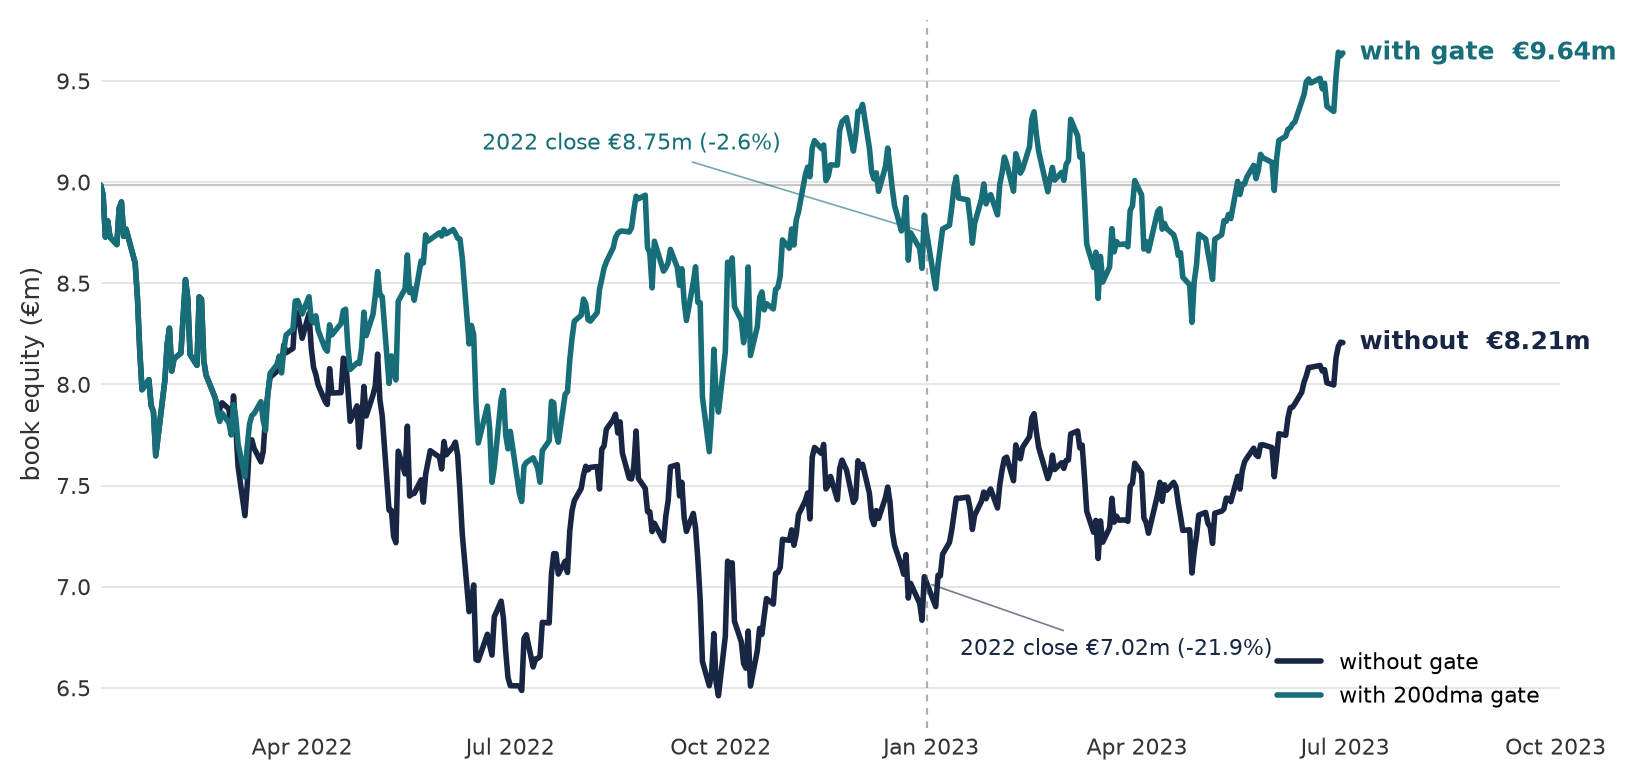
\includegraphics[width=0.98\textwidth]{bear_gate_curves.png}
\end{center}
\tabnote{The nine-name pooled book replayed through January 2022 -- June 2023 on
verified fills, deployed parameters, €9m starting capital: without protection
(navy) and with the 200dma gate (teal). The dashed line marks the 2022 year-end.}

The gate is not a hard floor --- positions already held when a name crosses under
its line still play out to target or stop, which is why 17.4\% of drawdown
remains. What it removes is the re-entry treadmill (fills 406 $\rightarrow$ 155,
stops 56 $\rightarrow$ 25), and what it adds is rotation: with the six AI names
gated, the pool concentrated the book's capital into VLO, CF and VST at full size
--- which the model traded to $+29\%$, $+49\%$ and $+29\%$ that year. The
$-2.6\%$ is early-leg losses on the AI names largely paid for by a fully-funded
good year in the diversifiers.

\section{What combination works best}

\subsection{The matrix}

\begin{center}
\begin{tabular}{lccccc}
\toprule
 & \multicolumn{2}{c}{calendar 2022} & \multicolumn{2}{c}{Jan 2022 -- Jun 2023} & bull cost \\
\cmidrule(lr){2-3}\cmidrule(lr){4-5}
config & return & max DD & total & max DD & (2024--26) \\
\midrule
nothing                          & $-21.9\%$ & 28.1\% & $-8.7\%$ & 28.1\% & --- \\
per-stock stop $-20\%$           & \multicolumn{4}{c}{treadmill continues}  & $\sim$10--15pp/yr \\
breaker 15\%/half                & $-18.2\%$ & 25.3\% & $-8.2\%$ & 25.3\% & 4.1pp/yr \\
\textbf{200dma gate}             & \good{$-2.6\%$} & \good{17.4\%} & \good{$+7.3\%$} & 17.4\% & \good{$\approx$0 pooled}$^{\dagger}$ \\
gate $+$ breaker                 & $-10.2\%$ & 20.9\% & $-1.1\%$ & 20.9\% & $\sim$4pp/yr \\
gate $+$ breaker $+$ stop $-25\%$& $-9.9\%$  & 20.4\% & $-0.9\%$ & 20.4\% & $\sim$4pp/yr \\
\bottomrule
\end{tabular}
\end{center}

\tabnote{Pooled book, equal weights, €9m, verified fills. Bull costs measured on
the 2024--26 sample; $^{\dagger}$the gate's pooled cost is $\approx$0 in return
terms but raises the April 2025 crash drawdown 29.2\% $\rightarrow$ 32.1\%
(concentration --- see \S4). Note the anti-synergy: the breaker stacked on the
gate makes the bear \emph{worse} because it half-sizes the diversifier entries
the gate has just concentrated capital into.}

\textbf{The answer is the gate, alone.} The mechanisms do not add --- they
interfere. The stop fires on accidents and charges rent on the best names; the
breaker's action is too blunt for a grind and sabotages the gate's rotation; the
gate both stops the treadmill \emph{and} redeploys the capital where the model is
still earning.

\subsection{Premium versus payout, and the frequency of bears}

Measured on the held construction the gate looked like classic expensive
insurance: $\sim$12pp/yr of premium against $\sim$19pp returned in a bear year
that arrives perhaps twice a decade --- a losing trade in expected value, worth
paying only for the drawdown control. The pooled measurement changes the
arithmetic: \textbf{in the loop the book actually trades, the premium is
approximately zero} (75.8\% vs 75.9\%/yr over 2024--26), because the pooling
reallocates gated capital instead of idling it. What the gate really costs is
not return but shape:

\begin{itemize}
\item \textbf{Concentration episodes in fast crashes.} April 2025: drawdown
29.2\% $\rightarrow$ 32.1\%, recovery three weeks later. This is the premium,
paid rarely and in drawdown rather than in return.
\item \textbf{Dependence on rotation targets.} The near-zero premium and the
2022 rescue both assume somewhere for gated capital to go. In a bear where
everything is gated, the book sits in cash at interest --- still
transformationally better than $-22\%$, but the diversifiers are what turn
``survive'' into ``flat''.
\item \textbf{What it buys}: $-21.9\% \rightarrow -2.6\%$ in the replayed bear
year, max drawdown 28.1\% $\rightarrow$ 17.4\%, and no recovery year needed ---
delivered precisely when capital is hardest to replace. With the premium at
approximately zero, insurance this cheap is bought, not debated; the alternative
defences are worse, and the volatility-based ones are proven counterproductive
(the overlays paper showed the model \emph{earns} from stress --- only direction
can be gated).
\end{itemize}

\subsection{The role of the diversifiers --- and the honest caveat}

The 2022 rescue had two parents: the gate stopped the bleeding, and the
diversifiers gave the freed capital somewhere to go. GM, VLO and CF were admitted
in 2026 partly on correlation grounds; the replay shows the mechanism working
exactly as intended, with the commodity trio carrying the book through an AI
winter. The caveat: 2022 happened to pair a growth bear with a commodity bull. In
a bear where \emph{everything} trades below its 200dma, the gate parks the book
in cash at interest --- still transformationally better than $-22\%$, but not
$-2.6\%$ either. The diversifiers are not a guarantee; they are an option the
gate knows how to exercise when it is there.

\section{Recommendation --- adopted}

\begin{tcolorbox}[colback=bcgold!8, colframe=bcgold, boxrule=0.8pt,
  title={\bfseries Adopted 15 August 2026}, coltitle=bcnavy]
\textbf{The 200dma gate, alone,} on all nine names: no new bids in a name whose
last close sits below its trailing 200-day average; exits untouched; freed
capital pools as normal. Wired into the live workbook the same day (\S7).
The circuit breaker is available as a \emph{fast-crash-only} satellite (trip
15\%, action half-size, reset on market signal or drawdown recovery --- never
full stand-down with an equity reset) but is not wired; the per-stock stop is
skipped.
\end{tcolorbox}

\section{Implementation in the live workbook}

The gate went live in the nine-stock workbook on 15 August 2026. The wiring is
layout-preserving by construction --- nothing was inserted or moved, so the order
block, the \texttt{IBKR\_Orders} range and the blotter keep their addresses and
the execution scripts read exactly what they read before. A full-workbook cell
diff against the pre-change file confirms every changed cell is an intended one,
and a Python mirror recomputed every 200dma, gate flag and ATH from the Query
data.

\subsection{The gate}

\begin{itemize}
\item \textbf{Active Trading, column N (``200 DMA''):} each order row carries its
stock's trailing 200-close average, computed directly off the Query close columns
with a COUNT-anchored window, so it tracks automatically as new rows are pasted
(expanding window until 200 closes exist).
\item \textbf{Allocation G25:G42 (``DMA gate''):} a per-sleeve flag --- 1 when the
stock's last close (Dashboard column B) sits below its 200dma (column N). The
flag is IFERROR-wrapped to \emph{fail open}: any lookup problem means ``no
gate'', never a dead sleeve.
\item \textbf{Allocation F25:F42:} the free-weight formula became
$E \times (1-\text{Held}) \times (1-\text{Gate})$. A gated sleeve drops out of
the cash renormalisation exactly like a HOLDING one, so its capital pools into
the ungated names' bids the same morning --- the mechanism behind the gate's
$\approx$0 pooled cost.
\item \textbf{What the scripts see:} a gated sleeve's order row shows Status
CASH, Tranche fund 0 and Qty 0. The one operational dependency: the order
script must skip zero-quantity BUY rows.
\end{itemize}

\subsection{The ATH-trap monitor}

Alongside the gate, Active Trading gained column O (``Sale \% below ATH''):
$(\text{ATH} - \text{sale})/\text{ATH}$, where the sale price is the row's live
one --- the calculated target on CASH rows, the actual resting sell on HOLDING
rows --- and the ATH is Dashboard column L. \textbf{A negative value means the
sale price sits above the all-time high}: the ATH trap identified in the August
review, now visible live on every order row. (VLO, whose close sits within
$\sim$1.3\% of its ATH with a $\sim$4\% OU premium, is the row most likely to
flag first.)

\subsection{State at adoption}

On the adoption date, one of the nine names opened gated: \textbf{VST} (close
146.40 against a 200dma of 161.37). Its two sleeves show fund 0 / Qty 0 and its
cash spreads across the other eight names --- the gate operating as designed, not
an error. The other eight names sat above their averages.

\section{Execution-accurate restatement (added 19 August)}

After this paper was issued, an execution fact was incorporated into the
research engine: the resting sell is a \emph{limit} order, so a held position
that gaps above its target overnight fills at the \emph{open}, not the target
--- every figure above books it at the target and is therefore conservative
(22\% of the book's held exits gapped over their targets in 2024--26). The
replay was re-run on the corrected basis. \textbf{Every conclusion and every
ordering in this paper is unchanged}; the levels move as follows.

\begin{center}
\begin{tabular}{lcccc}
\toprule
 & \multicolumn{2}{c}{calendar 2022} & \multicolumn{2}{c}{Jan 2022 -- Jun 2023} \\
\cmidrule(lr){2-3}\cmidrule(lr){4-5}
config (exec.-accurate) & return & max DD & total & max DD \\
\midrule
nothing            & $-20.1\%$ & 27.4\% & $-3.3\%$  & 27.4\% \\
\textbf{200dma gate} & \good{$-1.3\%$} & \good{16.9\%} & \good{$+13.0\%$} & 16.9\% \\
breaker 15\%/half  & $-16.8\%$ & 24.8\% & $-2.9\%$  & 24.8\% \\
gate $+$ breaker   & $-9.7\%$  & 20.0\% & $+3.4\%$  & 20.0\% \\
\bottomrule
\end{tabular}
\end{center}

\tabnote{Compare \S5: the corrections are small in the bear year (a falling
tape produces few overnight gaps above targets) and favour the gate slightly
--- its 2022 outcome improves to $-1.3\%$ and its Jan~2022--Jun~2023 total to
$+13.0\%$. On the bull side (2024--26, no pre-market rule, matching \S4's
basis) the corrected pooled book runs 91.4\%/yr without the gate and
93.3\%/yr with it --- the gate's $\approx$zero pooled cost is confirmed and
now mildly positive --- while the April 2025 concentration episode persists
unchanged in character ($-28.7\%$ ungated vs $-31.8\%$ gated). The
recommendation stands exactly as adopted.}

\section{The breadth upgrade: gate on the bear, not the name (added 26 August)}

\subsection{The live observation that prompted it}

Eleven days into live operation the gate showed its one designed-in cost in
real time: \textbf{VST sat below its 200dma while recovering from its own
drawdown, gated} --- and visibly missing the recovery fills the model exists to
harvest. The gate was built against 2022, where the \emph{book} broke down; a
lone name below its line is usually not that event. The question (the user's):
should the gate fire only when \emph{several} names breach at once --- breadth
as the bear signal?

\subsection{The rule, and the diagnostic that justifies it}

Per name, each morning, strictly ex ante: \emph{a stock below its own 200dma is
gated only when at least $K$ of the nine names are below theirs}. $K{=}1$
reproduces the per-name gate of \S4.

The 2024--26 sample splits exactly the way the intuition says it should.
Breaches are overwhelmingly \textbf{isolated}: 193 days with exactly one name
below its line and 171 with two, against only 60 days at breadth ${\ge}5$ (the
April 2025 episode). And the trades the per-name gate refused on those isolated
days were \emph{good} trades: reconstructing all 384 forgone entries at breadth
$<3$ and following each to its exit, they averaged \good{$+2.35\%$} (median
$+2.54\%$, 21 losers of 384) --- ordinary harvest, taxed. VST alone accounts for
195 gated days and 129 of those forgone entries. In 2022, by contrast, breadth
\emph{was} the event: 144 trading days had six names below their lines at once.

\subsection{Both regimes, priced}

\begin{center}
\begin{tabular}{lccccc}
\toprule
 & \multicolumn{3}{c}{2024--26 (pooled, live config)} & \multicolumn{2}{c}{calendar 2022} \\
\cmidrule(lr){2-4}\cmidrule(lr){5-6}
config & train & test & max DD & return & max DD \\
\midrule
no gate            & 59.5\% & 118.4\% & 25.8\% & $-21.9\%$ & 28.1\% \\
per-name gate (\S4) & 59.4\% & 119.0\% & \bad{32.2\%} & \good{$-2.6\%$} & 17.4\% \\
\textbf{breadth $K{=}4$} & \good{64.6\%} & 117.3\% & \good{25.8\%} & \good{$-2.6\%$} & 17.4\% \\
breadth $K{=}5$    & 71.1\% & 117.4\% & 21.7\% & \good{$-0.4\%$} & 16.1\% \\
breadth $K{=}6$    & 71.1\% & 117.4\% & 21.7\% & \bad{$-12.6\%$} & 23.2\% \\
\bottomrule
\end{tabular}
\end{center}

\tabnote{2024--26 on the live configuration (9:00/4\% pre-market rule active on
both sides, sheet exit convention), both halves of the standard split; the
max-DD column is dominated by the April 2025 episode. 2022 as in \S5 (no
pre-market data exists pre-2024). Orderings, not levels, carry between bases.}

Three facts decide it. \textbf{First, the 2022 protection is fully preserved
through $K{=}4$} --- identical to the per-name gate to the decimal, because the
real bear was a breadth event. \textbf{Second, breadth-conditioning fixes the
April 2025 concentration penalty of \S4}: the per-name gate spent the long
single-name run-up and recovery tails starving the pool (drawdown 25.8\%
$\rightarrow$ 32.2\%); the breadth gate fires only during the acute broad phase
and the episode returns to 25.8\% at $K{=}4$ (21.7\% at $K{=}5$). \textbf{Third,
the protection boundary is $K \le 5$}: 2022's plateau was exactly six names
below (the three diversifiers held up), so $K{=}6$ forfeits the early-decline
protection ($-12.6\%$) --- a cliff, not a slope.

\subsection{Choosing K, and the adoption}

$K{=}5$ is the best cell everywhere in sample but sits one step from that
cliff: a future bear in which one more diversifier holds up would peak at
breadth five and $K{=}5$ would catch it with no margin. $K{=}4$ keeps
\textbf{two names of headroom}, retains the full 2022 save, removes the April
concentration penalty, and collects $+5.2$pp of train-half return against a
$-1.7$pp tested-half difference that is within noise --- and since the gate's
product is drawdown control, drawdown dominance at $\approx$zero return cost is
the deciding comparison.

\begin{tcolorbox}[colback=bcgold!8, colframe=bcgold, boxrule=0.8pt,
  title={\bfseries Adopted 26 August 2026 --- the gate becomes breadth-conditional, $K=4$},
  coltitle=bcnavy]
A stock below its own 200-day average is gated \textbf{only when at least four
of the nine names are below theirs}. An isolated breach --- a name recovering
from its own drawdown --- trades normally. Wired the same day
(\texttt{wire\_breadth\_gate.py}, cell-diff verified): Active Trading M8 holds
$K$ (Gate Variables block); Allocation G43 counts the names currently below
(column G keeps the raw per-name flags); F25:F42 apply the gate as
$\text{breach} \times (\text{G43} \ge K)$. A blank M8 \emph{fails closed} to
the per-name gate --- the failure direction is more protection, never less.
Column N's traffic lights are unchanged: red still means ``below its own
line''; whether red is \emph{enforced} is read by comparing G43 with M8.
\end{tcolorbox}

At wiring, the live state was breadth 2 (VST and RKLB below): the gate stood
unarmed and both names' recovery bids went back into the morning allocation ---
the exact leak the observation identified, closed.

\section{Composition note: RKLB out, AVGO in (2 September 2026)}

AVGO replaced RKLB in the book on 2 September 2026 --- a risk decision by the
principal (SpaceX-linked performance, binary launch events), recorded in full
in the ranking memo. What it means for this paper:

\textbf{The machinery carries over untouched.} Every mechanism here is
book-level and name-agnostic: the 50-day stop, the circuit breaker, the
per-name 200dma test and the breadth condition are wired by \emph{slot}, not
by ticker. Allocation G43 counts whichever nine names occupy the slots, so
AVGO's breach flag entered the breadth count the moment it entered the book;
$K{=}4$ and the fail-closed direction are unchanged. Nothing in \S1--\S9
needed rewiring.

\textbf{The measurements are of the RKLB-era book.} The 2022 replay table
(\S1), the protection matrix (\S6) and the April 2025 stress reading are
measurements of the roster that included RKLB --- including the episode where
the pooled loop concentrated into RKLB as the one name still above its line
(\S6). That concentration \emph{channel} survives the swap (the pool will
always crowd the last names standing); its worst actor does not. On the
2024--26 sample the swapped book's maximum drawdown improves 25.8\% $\to$
24.7\%.

\textbf{What is pending.} A 2022 replay of the \emph{current} roster needs
AVGO 5-minute bars for Aug 2021 -- Jun 2023 (same Box format as the other
nine); the re-run is queued on that data. The unverified expectation, stated
for the record and to be tested, is that the swap softens the unprotected
2022 result --- AVGO's public-record 2022 drawdown was materially shallower
than RKLB's (roughly $-40\%$ against $-80\%$) --- while the gated result
should remain near flat since the gate's save came from the diversifiers.
Until that replay runs, the 2022 numbers in this paper stand as evidence for
the \emph{mechanisms}, not as forecasts for the current roster.

\vspace{0.4cm}
{\color{bcnavy}\hrule height 0.8pt}
\vspace{0.2cm}
{\footnotesize\color{bcgrey} Basis: bear side --- user-supplied 5-minute bars
Aug 2021 -- Jun 2023 for all nine names, deployed 2024--26 parameters replayed
with verified fills, pooled equal-weight book, €9m; bull side --- the standard
2024--26 verified sample. Interest on idle cash held at the model's 3.14\%/yr
throughout (understates 2022 cash income). Scripts:
\texttt{bear\_replay.py}, \texttt{price\_stop\_study.py}, \texttt{book\_sim.py}
(breaker, price-stop and gate support), \texttt{breadth\_gate.py} (\S9);
workbook wiring \texttt{wire\_200dma.py} and \texttt{wire\_breadth\_gate.py}
(re-runnable on any future copy). Findings recorded in HANDOVER \S3.13 and
\S3.23. Companion paper: \emph{Three Volatility Overlays, Tested and
Rejected} (14 Aug 2026).}

\end{document}
